%==============================================================================
%  STAT 412 -- Homework 1 -- ANSWER KEY  (paste-ready, self-contained)
%
%  Upload the matching screenshots alongside this file (same folder) so the
%  \includegraphics paths resolve.
%
%  NOTE: Questions 7--20 had no usable source material (all source files were
%  empty / 0-byte). Only Questions 1--6 could be transcribed and solved; they
%  appear below. Re-capture the missing screenshots to extend this key.
%==============================================================================
\documentclass[11pt]{article}

\usepackage[margin=1in]{geometry}
\usepackage{amsmath,amssymb}
\usepackage{graphicx}
\usepackage{float}
\usepackage{booktabs}
\usepackage{siunitx}
\usepackage{enumitem}
\usepackage{pifont}
\usepackage[dvipsnames]{xcolor}
\usepackage{tcolorbox}
\usepackage{fancyhdr}
\usepackage{caption}
\usepackage{hyperref}
\hypersetup{colorlinks=true,linkcolor=NavyBlue,urlcolor=NavyBlue}

\captionsetup{font=small,labelfont=bf}

% --- answer box used to highlight the final answer of each question ----------
\newtcolorbox{answerbox}{colback=Green!6,colframe=Green!55!black,
  boxrule=0.8pt,arc=2pt,left=8pt,right=8pt,top=6pt,bottom=6pt}

% --- running header ---------------------------------------------------------
\pagestyle{fancy}
\fancyhf{}
\lhead{\small STAT 412 — Homework 1}
\rhead{\small Answer Key}
\cfoot{\small\thepage}
\renewcommand{\headrulewidth}{0.4pt}

\title{\vspace{-1.5em}\textbf{STAT 412 — Homework 1}\\[2pt]
       \large Answer Key with Full Solutions}
\author{}
\date{}

\begin{document}
\maketitle
\thispagestyle{fancy}
\vspace{-2.5em}

%==============================================================================
\section{Comparative Dotplot of Rubber Tensile Strength}
%==============================================================================

\subsection*{Problem}
The tensile strength of silicone rubber is thought to be a function of curing
temperature. A study was carried out in which $12$ specimens of the rubber were
prepared using each of two curing temperatures, \SI{20}{\celsius} and
\SI{45}{\celsius}. The resulting tensile-strength measurements (MPa) are:

\begin{table}[H]
\centering
\renewcommand{\arraystretch}{1.25}
\begin{tabular}{l *{12}{c}}
\toprule
\textbf{\SI{20}{\celsius} (Low)}
 & 2.07 & 2.19 & 2.29 & 2.04 & 2.24 & 2.04
 & 2.09 & 2.18 & 2.02 & 2.19 & 2.16 & 2.05 \\
\textbf{\SI{45}{\celsius} (High)}
 & 2.42 & 2.16 & 2.44 & 2.04 & 2.37 & 2.09
 & 1.96 & 2.49 & 2.08 & 2.49 & 2.25 & 2.01 \\
\bottomrule
\end{tabular}
\caption{Rubber tensile strengths at the two curing temperatures.}
\end{table}

\subsection*{Part (a) — Show a dotplot of the data (low and high temperature)}

\noindent
Four candidate comparative dotplots (a–d) are shown below, in which
\textcolor{blue}{$\circ$} = Low temperature (\SI{20}{\celsius}) and
\textcolor{red}{$\times$} = High temperature (\SI{45}{\celsius}).
\textbf{Which dotplot correctly displays the data?}

\begin{figure}[H]
\centering
\begin{minipage}{0.48\textwidth}\centering
  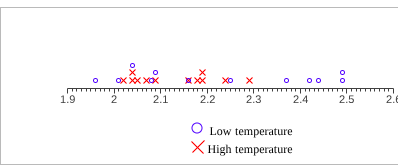
\includegraphics[width=\linewidth]{q1_dotplot_a.png}
  \caption*{\textbf{(a)}}
\end{minipage}\hfill
\begin{minipage}{0.48\textwidth}\centering
  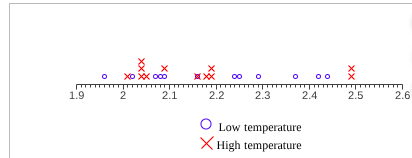
\includegraphics[width=\linewidth]{q1_dotplot_b.png}
  \caption*{\textbf{(b)}}
\end{minipage}

\vspace{0.6em}
\begin{minipage}{0.48\textwidth}\centering
  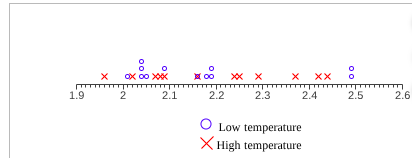
\includegraphics[width=\linewidth]{q1_dotplot_c.png}
  \caption*{\textbf{(c)}}
\end{minipage}\hfill
\begin{minipage}{0.48\textwidth}\centering
  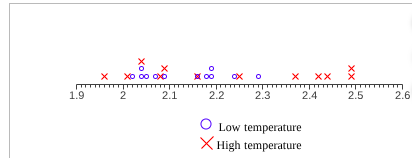
\includegraphics[width=\linewidth]{q1_dotplot_d.png}
  \caption*{\textbf{(d)}}
\end{minipage}
\caption{The four candidate comparative dotplots.}
\end{figure}

\paragraph{Step 1: Sort each group.}
\[
\begin{aligned}
\textbf{Low }(\SI{20}{\celsius}):\;
 & 2.02,\,2.04,\,2.04,\,2.05,\,2.07,\,2.09,\,2.16,\,2.18,\,2.19,\,2.19,\,2.24,\,2.29\\
\textbf{High }(\SI{45}{\celsius}):\;
 & 1.96,\,2.01,\,2.04,\,2.08,\,2.09,\,2.16,\,2.25,\,2.37,\,2.42,\,2.44,\,2.49,\,2.49
\end{aligned}
\]

\paragraph{Step 2: Use the two extremes as ``fingerprints.''}
\begin{itemize}[leftmargin=1.4em]
  \item \textbf{Overall minimum $=1.96$} belongs to the \emph{High} group, so the
        single left-most mark must be a \textcolor{red}{red $\times$}.
  \item \textbf{Overall maximum $=2.49$ (twice)} also belongs to the \emph{High}
        group, so the two right-most marks must be \textcolor{red}{red $\times$}'s.
  \item The \emph{Low} group never goes below $2.02$ or above $2.29$, so
        \textbf{no \textcolor{blue}{blue $\circ$} may appear at either extreme.}
\end{itemize}

\paragraph{Step 3: Test each option against the fingerprints.}
\begin{table}[H]
\centering
\renewcommand{\arraystretch}{1.3}
\begin{tabular}{c l l c}
\toprule
Plot & Left-most mark ($\approx1.96$) & Right-most marks ($\approx2.49$) & Verdict \\
\midrule
(a) & \textcolor{blue}{$\circ$} (blue)  & \textcolor{blue}{$\circ$} (blue)  & \ding{55}\ colors swapped \\
(b) & \textcolor{blue}{$\circ$} (blue)  & \textcolor{red}{$\times$} (red)   & \ding{55}\ min wrong color \\
(c) & \textcolor{red}{$\times$} (red)   & \textcolor{blue}{$\circ$} (blue)  & \ding{55}\ max wrong color \\
(d) & \textcolor{red}{$\times$} (red)   & \textcolor{red}{$\times$} (red)   & \checkmark\ matches data \\
\bottomrule
\end{tabular}
\caption{Only plot (d) places both extremes in the High-temperature group.}
\end{table}

\noindent
Only \textbf{plot (d)} puts the smallest value \emph{and} the two largest values
in the High group, with the Low group confined to the $2.02$–$2.29$ band.

\begin{answerbox}
\textbf{Answer (a): Dot plot (d)} is the correct comparative dotplot.
\end{answerbox}

\subsection*{Part (b) — Sample mean tensile strength for each group}

\paragraph{Low temperature (\SI{20}{\celsius}).} Sum $=25.56$, so
\[
\bar{x}_{\text{low}}=\frac{25.56}{12}=2.130 .
\]

\paragraph{High temperature (\SI{45}{\celsius}).} Sum $=26.80$, so
\[
\bar{x}_{\text{high}}=\frac{26.80}{12}=2.2333\ldots\approx 2.233 .
\]

\begin{answerbox}
\textbf{Answer (b):}\quad
$\bar{x}_{\text{low}} = 2.130$ MPa \qquad
$\bar{x}_{\text{high}} = 2.233$ MPa \quad(rounded to three decimals).
\end{answerbox}

\subsection*{Part (c) — Does curing temperature affect tensile strength?}

\noindent
\begin{enumerate}[label=\textbf{\Alph*.},leftmargin=2.2em,itemsep=2pt]
  \item Yes. The high-temperature observations are generally \emph{lower}.
  \item Yes. The high-temperature observations are generally \emph{higher}.
  \item No. The two groups are similar.
  \item No. The plot cannot distinguish the two groups.
\end{enumerate}

\noindent
The high-temperature group has the larger center ($\bar{x}=2.233$ vs.\ $2.130$,
median $2.205$ vs.\ $2.125$) and holds all the largest values ($2.37$–$2.49$).

\begin{answerbox}
\textbf{Answer (c): B} --- Yes; the high-temperature observations are generally
higher, so curing temperature appears to increase tensile strength.
\end{answerbox}

\subsection*{Part (d) — Is anything else influenced by curing temperature?}

\noindent
\begin{enumerate}[label=\textbf{\Alph*.},leftmargin=2.2em,itemsep=2pt]
  \item Yes. Higher temperature leads to a \emph{decrease} in variability.
  \item Yes. Higher temperature leads to an \emph{increase} in variability.
  \item No. The variability is similar in both groups.
  \item No. The plot cannot distinguish the two groups.
\end{enumerate}

\noindent
The high-temperature group contains \emph{both} the smallest value ($1.96$) and
the two largest ($2.49$), so its range is nearly double:
\[
R_{\text{high}}=2.49-1.96=0.53 \;>\; R_{\text{low}}=2.29-2.02=0.27 .
\]

\begin{answerbox}
\textbf{Answer (d): B} --- Yes; the high-temperature group is more spread out, so
an increase in curing temperature increases the variability.
\end{answerbox}

\subsection*{Summary}
\begin{center}
\renewcommand{\arraystretch}{1.25}
\begin{tabular}{l c c c c}
\toprule
Group & Mean & Median & Range & Spread \\
\midrule
Low (\SI{20}{\celsius})  & $2.130$ & $2.125$ & $0.27$ & tight cluster \\
High (\SI{45}{\celsius}) & $2.233$ & $2.205$ & $0.53$ & much wider \\
\bottomrule
\end{tabular}
\end{center}

%==============================================================================
\section{Flexibility of Springs --- Two Suppliers}
%==============================================================================

\subsection*{Problem}
Steel rods from two companies were compared; ten sample springs were made from
each company's rods and a flexibility measure recorded for each. Complete parts
(a) and (b).

\begin{table}[H]
\centering
\renewcommand{\arraystretch}{1.25}
\begin{tabular}{l *{10}{c}}
\toprule
\textbf{Company A} & 8.8 & 8.4 & 6.7 & 8.2 & 8.1 & 7.3 & 7.8 & 6.6 & 9.1 & 6.5 \\
\textbf{Company B} & 10.5 & 10.2 & 10.1 & 10.3 & 10.4 & 9.6 & 10.5 & 11.1 & 10.3 & 9.9 \\
\bottomrule
\end{tabular}
\caption{Flexibility of springs ($n=10$ per company).}
\end{table}

\subsection*{Part (a) — Sample mean and median for each company}

\paragraph{Sorted data.}
\[
\begin{aligned}
\text{A}:\;& 6.5,\,6.6,\,6.7,\,7.3,\,\underline{7.8},\,\underline{8.1},\,8.2,\,8.4,\,8.8,\,9.1\\
\text{B}:\;& 9.6,\,9.9,\,10.1,\,10.2,\,\underline{10.3},\,\underline{10.3},\,10.4,\,10.5,\,10.5,\,11.1
\end{aligned}
\]

\paragraph{Means.}
\[
\bar{x}_A=\frac{77.5}{10}=7.75,\qquad \bar{x}_B=\frac{102.9}{10}=10.29 .
\]

\paragraph{Medians} (average of the 5th and 6th ordered values).
\[
\tilde{x}_A=\frac{7.8+8.1}{2}=7.95,\qquad \tilde{x}_B=\frac{10.3+10.3}{2}=10.30 .
\]

\begin{answerbox}
\textbf{Answer (a):}\quad
Company A: mean $=7.75$, median $=7.95$.\\
\hphantom{\textbf{Answer (a):}\quad}
Company B: mean $=10.29$, median $=10.30$.
\end{answerbox}

\subsection*{Part (b) — Plot the data and describe any differences}

\noindent
\textbf{(b.1) Which dotplot correctly displays the data?}\\
Four candidate dotplots are shown below, with
\textcolor{blue}{$\circ$} = Company A and \textcolor{red}{$\times$} = Company B.

\begin{figure}[H]
\centering
\begin{minipage}{0.48\textwidth}\centering
  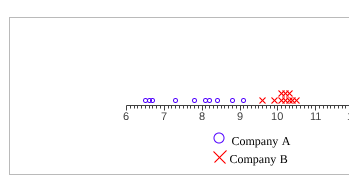
\includegraphics[width=\linewidth]{q2_dotplot_a.png}
  \caption*{\textbf{(a)}}
\end{minipage}\hfill
\begin{minipage}{0.48\textwidth}\centering
  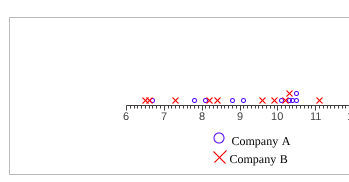
\includegraphics[width=\linewidth]{q2_dotplot_b.png}
  \caption*{\textbf{(b)}}
\end{minipage}

\vspace{0.6em}
\begin{minipage}{0.48\textwidth}\centering
  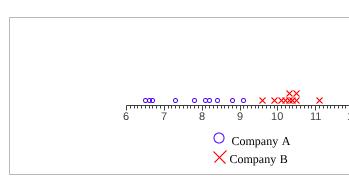
\includegraphics[width=\linewidth]{q2_dotplot_c.png}
  \caption*{\textbf{(c)}}
\end{minipage}\hfill
\begin{minipage}{0.48\textwidth}\centering
  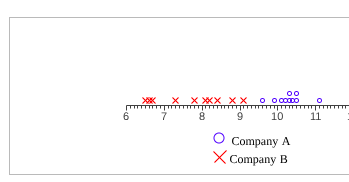
\includegraphics[width=\linewidth]{q2_dotplot_d.png}
  \caption*{\textbf{(d)}}
\end{minipage}
\caption{The four candidate dotplots of spring flexibility.}
\end{figure}

\paragraph{Key features.}
Company A ranges $6.5$–$9.1$; Company B ranges $9.6$–$11.1$. The correct plot must
show (i) blue $\circ$ on the left and red $\times$ on the right with almost no
overlap, and (ii) Company B's maximum $11.1$ as an \emph{isolated} red $\times$ to
the right of its $10.1$–$10.5$ cluster (which has double stacks at $10.3$, $10.5$).

\begin{table}[H]
\centering
\renewcommand{\arraystretch}{1.3}
\begin{tabular}{c p{0.62\textwidth} c}
\toprule
Plot & \multicolumn{1}{c}{What it shows} & Verdict \\
\midrule
(a) & reds stop at $\approx10.5$ (no isolated $11.1$); wrong triple-stack & \ding{55} \\
(b) & blue and red intermixed across the whole axis & \ding{55} \\
(c) & blue left, red right; isolated red at $11.1$; stacks at $10.3,10.5$ & \checkmark \\
(d) & colors swapped (red on the left, blue on the right) & \ding{55} \\
\bottomrule
\end{tabular}
\caption{Only plot (c) reproduces the separation and Company B's isolated maximum.}
\end{table}

\noindent
Only \textbf{plot (c)} matches both features.

\begin{answerbox}
\textbf{Answer (b.1): Dot plot (c)} is correct. Company A's values (6.5 to 9.1)
sit to the left and Company B's (9.6 to 11.1) to the right, with B's largest
value, 11.1, isolated from its 10.1--10.5 cluster.
\end{answerbox}

\medskip
\noindent
\textbf{(b.2) Give your impression of any apparent differences. Choose the
correct answer below.}
\begin{enumerate}[label=\textbf{\Alph*.},leftmargin=2.2em,itemsep=3pt]
  \item The rods from Company B have a lower measure of flexibility than the rods
        from Company A, since the data points for Company A are farther to the
        right on the line.
  \item The rods from both companies have about the same flexibility, since the
        data points for the two companies are mixed together.
  \item The rods from Company B have a higher measure of flexibility than the rods
        from Company A, since the data points for Company B are farther to the
        right on the line.
\end{enumerate}

\noindent
The dotplot and the means agree: Company B's marks sit entirely to the right of
Company A's ($\bar{x}_B=10.29 > \bar{x}_A=7.75$), so Company B's rods are more
flexible.

\begin{answerbox}
\textbf{Answer (b.2): C} --- Company B has a higher measure of flexibility than
Company A, since Company B's data points are farther to the right on the line.
\end{answerbox}

%==============================================================================
\section{Flexibility of Springs --- Mean and Variance}
%==============================================================================

\subsection*{Problem}
Same two-company setup, a \emph{new} sample of ten springs each. Compute the
\textbf{mean} and \textbf{variance} in flexibility for both companies and decide
whether flexibility appears to differ.

\begin{table}[H]
\centering
\renewcommand{\arraystretch}{1.25}
\begin{tabular}{l *{10}{c}}
\toprule
\textbf{Company A} & 9.2 & 8.3 & 6.6 & 8.9 & 8.6 & 6.8 & 8.4 & 6.1 & 8.5 & 7.1 \\
\textbf{Company B} & 10.7 & 10.5 & 9.8 & 9.9 & 9.7 & 9.6 & 10.7 & 10.8 & 9.9 & 9.6 \\
\bottomrule
\end{tabular}
\caption{Flexibility of springs ($n=10$ per company).}
\end{table}

\subsection*{Solution}

\paragraph{Means.}
\[
\bar{x}_A=\frac{78.5}{10}=7.8500,\qquad \bar{x}_B=\frac{101.2}{10}=10.1200 .
\]

\paragraph{Variances} (sample variance, $s^2=\tfrac{1}{n-1}\sum (x_i-\bar{x})^2$, $n-1=9$).
\[
s_A^2=\frac{10.7050}{9}=1.1894,\qquad s_B^2=\frac{2.1960}{9}=0.2440 .
\]

\begin{answerbox}
\textbf{Answer (mean \& variance):}\quad
Company A: mean $=7.8500$, variance $=1.1894$.\\
\hphantom{\textbf{Answer (mean \& variance):}\quad}
Company B: mean $=10.1200$, variance $=0.2440$.
\end{answerbox}

\subsection*{Does flexibility differ? — complete the statement}

\noindent
The problem asks you to fill three dropdowns. Comparing the computed values:
\[
\bar{x}_A = 7.8500 \;<\; \bar{x}_B = 10.1200,
\qquad
s_A^2 = 1.1894 \;>\; s_B^2 = 0.2440 .
\]

\begin{answerbox}
\textbf{Answer:} There \textbf{does appear} to be a difference in flexibility.
Company A's sample mean is \textbf{smaller than} company B's sample mean, and
company A's variance is \textbf{greater than} company B's variance.
\end{answerbox}

\noindent
\emph{Interpretation.} Company~B's rods are more flexible on average \emph{and}
more consistent (smaller variance); Company~A's are less flexible and more
variable --- so the companies clearly differ.

\medskip
\noindent\footnotesize\emph{Note.} If population variance is wanted ($\div n$):
$\sigma_A^2 = 10.7050/10 = 1.0705$, $\sigma_B^2 = 2.1960/10 = 0.2196$.

%==============================================================================
\section{Tensile Strength --- Standard Deviation by Temperature}
%==============================================================================

\subsection*{Problem}
A new rubber tensile-strength study, $12$ specimens at each of \SI{20}{\celsius}
and \SI{45}{\celsius}. Compute the sample standard deviation for each temperature
and decide whether an increase in temperature influences the \emph{variability}.

\begin{table}[H]
\centering
\renewcommand{\arraystretch}{1.25}
\begin{tabular}{l *{12}{c}}
\toprule
\textbf{\SI{20}{\celsius} (Low)}
 & 2.05 & 2.11 & 2.29 & 2.04 & 2.23 & 2.04 & 2.08 & 2.15 & 2.06 & 2.11 & 2.18 & 2.01 \\
\textbf{\SI{45}{\celsius} (High)}
 & 2.42 & 2.17 & 2.46 & 2.04 & 2.39 & 2.08 & 1.97 & 2.45 & 2.09 & 2.45 & 2.28 & 2.07 \\
\bottomrule
\end{tabular}
\caption{Tensile strengths (MPa), $n=12$ per temperature.}
\end{table}

\subsection*{Part (a) — Sample standard deviation for each group}

\noindent
Using $s=\sqrt{\dfrac{1}{n-1}\sum (x_i-\bar{x})^2}$ with $n=12$
($\bar{x}_{\text{low}}=2.1125$, $\bar{x}_{\text{high}}=2.2392$):
\[
s_{\text{low}}=0.0853,\qquad s_{\text{high}}=0.1878
\quad\text{(4 d.p.)}.
\]

\begin{answerbox}
\textbf{Answer (a):}\quad
$s_{\text{low}} = 0.0853$ MPa \qquad $s_{\text{high}} = 0.1878$ MPa.
\end{answerbox}

\noindent
\textbf{Does temperature influence variability?} \emph{Yes.} The high-temperature
standard deviation ($0.1878$) is more than double the low-temperature one
($0.0853$), so an increase in curing temperature appears to \emph{increase} the
variability in tensile strength.

%-- Q4 parts (b)+ to be added when their prompts are available ----------------

%==============================================================================
\section{Smoking and Sleep Patterns}
%==============================================================================

\subsection*{Problem}
Time (minutes) to fall asleep is recorded for smokers and nonsmokers. Complete
parts (a)–(d).

\begin{table}[H]
\centering
\renewcommand{\arraystretch}{1.25}
\resizebox{\textwidth}{!}{%
\begin{tabular}{l *{12}{c}}
\toprule
\textbf{Smokers} ($n{=}11$)
 & 69.3 & 56.0 & 22.1 & 47.6 & 53.2 & 48.1 & 34.4 & 60.2 & 43.8 & 23.2 & 13.8 & \\
\textbf{Nonsmokers} ($n{=}12$)
 & 28.6 & 25.1 & 26.4 & 34.9 & 29.8 & 38.5 & 30.2 & 30.6 & 31.8 & 41.6 & 21.1 & 37.9 \\
\bottomrule
\end{tabular}}
\caption{Minutes to fall asleep.}
\end{table}

\subsection*{Part (a) — Sample mean for each group}
\[
\bar{x}_{\text{smokers}}=\frac{471.7}{11}=42.88,\qquad
\bar{x}_{\text{nonsmokers}}=\frac{376.5}{12}=31.38
\quad\text{(2 d.p.)}.
\]

\begin{answerbox}
\textbf{Answer (a):}\quad
Smokers: $42.88$ min \qquad Nonsmokers: $31.38$ min.
\end{answerbox}

\subsection*{Part (b) — Sample standard deviation for each group}
\[
s_{\text{smokers}}=\sqrt{\frac{\sum (x_i-42.88)^2}{10}}=17.50,\qquad
s_{\text{nonsmokers}}=\sqrt{\frac{\sum (x_i-31.38)^2}{11}}=5.97
\quad\text{(2 d.p.)}.
\]

\begin{answerbox}
\textbf{Answer (b):}\quad
Smokers: $s=17.50$ min \qquad Nonsmokers: $s=5.97$ min.
\end{answerbox}

\noindent
Smokers not only take longer to fall asleep on average but are far more variable
($s=17.50$ vs.\ $5.97$ minutes).

%-- Q5 parts (c)-(d) to be added when their prompts are available -------------

%==============================================================================
\section{Teacher Salaries (Dollars per Pupil)}
%==============================================================================

\subsection*{Problem}
Historical staff-salary data (\$/pupil) for $30$ schools. Complete parts (a)–(c).

\begin{table}[H]
\centering
\renewcommand{\arraystretch}{1.2}
\begin{tabular}{*{10}{c}}
\toprule
3.94 & 2.91 & 2.82 & 2.83 & 3.05 & 1.77 & 2.46 & 3.12 & 2.36 & 2.07 \\
2.73 & 2.57 & 2.76 & 2.70 & 3.66 & 3.82 & 3.33 & 2.04 & 2.89 & 2.85 \\
3.24 & 2.44 & 2.09 & 3.73 & 3.07 & 3.53 & 2.30 & 2.59 & 3.59 & 3.34 \\
\bottomrule
\end{tabular}
\caption{Staff salaries (\$/pupil), $n=30$.}
\end{table}

\subsection*{Part (a) — Sample mean and sample standard deviation}
\[
\bar{x}=\frac{86.60}{30}=2.8867,\qquad
s=\sqrt{\frac{\sum (x_i-\bar{x})^2}{29}}=0.5688
\quad\text{(4 d.p.)}.
\]

\begin{answerbox}
\textbf{Answer (a):}\quad
mean $=2.8867$ \qquad standard deviation $=0.5688$.
\end{answerbox}

\subsection*{Part (b) — Relative frequency histogram}

\noindent
Grouping the $30$ salaries into classes of width $0.5$ gives the relative
frequencies below (computed and plotted in Python):

\begin{table}[H]
\centering
\renewcommand{\arraystretch}{1.2}
\begin{tabular}{l c c c c c}
\toprule
Class ($\$/$pupil) & $[1.5,2.0)$ & $[2.0,2.5)$ & $[2.5,3.0)$ & $[3.0,3.5)$ & $[3.5,4.0)$ \\
\midrule
Frequency           & 1      & 7      & 10     & 6      & 6 \\
Relative frequency  & 0.0333 & 0.2333 & 0.3333 & 0.2000 & 0.2000 \\
\bottomrule
\end{tabular}
\caption{Relative-frequency distribution of staff salaries.}
\end{table}

\begin{figure}[H]
\centering
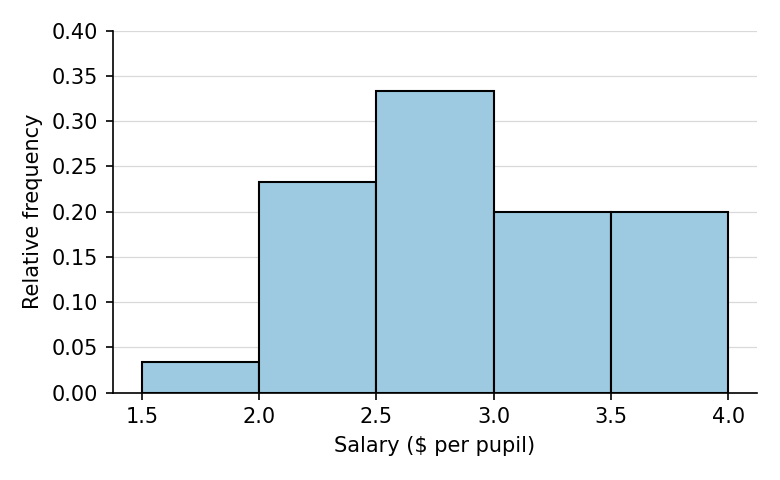
\includegraphics[width=0.62\textwidth]{q6_histogram.png}
\caption{Relative frequency histogram (the correct choice). It is unimodal with
its peak in the $[2.5,3.0)$ class, rising from a low $[1.5,2.0)$ bar and tapering
to a flat right tail.}
\end{figure}

\begin{answerbox}
\textbf{Answer (b):} Choose the histogram that is \textbf{unimodal with its tallest
bar over $[2.5,3.0)$} (relative frequency $\approx0.33$), a short bar at
$[1.5,2.0)$ ($\approx0.03$), and equal $0.20$ bars over $[3.0,3.5)$ and
$[3.5,4.0)$ --- matching Figure~5 above.
\end{answerbox}

%-- Q6 part (c) to be added when its prompt is available ----------------------

\end{document}
